\section{Metolodgía de trabajo}

Nursoft se ha desenvuelto a lo largo de su vida en más de 20 proyectos de desarrollo de software. 
Los rubros de cada proyecto se extienden desde la minería, pasando por \textit{retail}, industria agropecuaria, 
mercado inmobiliario, \textit{e-learning} hasta en tele-medicina. 

Una mayoría importante de los proyectos caen en lo que es
\textbf{desarrollo de software clásico}, y el resto son entendidos como \textbf{consultorías}:
estos son proyectos donde el cliente está interesado inicialmente en conocer la factibilidad,
tanto comercial como técnica, de alguna propuesta o solución tecnológica generada por terceros o ellos mismos.

El primer grupo de proyectos se puede ceñir a una estructura informal de procesos como la siguiente:

\begin{itemize}
  \item Cliente presenta su necesidad/problema
  \item Nursoft indaga el estado actual del cliente para contextualizar la necesidad/problema
  \item Nursoft propone una solución
  \item Se realiza la planificación (junto con diseños necesarios)
  \item Se realiza la implementación
  \item Se realizan entregas periódicas
\end{itemize}

Por otro lado, las consultorías se ciñen a la siguiente estructura de procesos:

\begin{itemize}
  \item Cliente presenta su necesidad/problema junto con su propuesta
  \item Nursoft indaga el estado actual del cliente para contextualizar la necesidad/problema y la propuesta entregada
  \item Nursoft propone una contra-propuesta o modifica la propuesta entregada
  \item Nursoft valida la factibilidad comercial
  \item Nursoft valida la factibilidad técnica
\end{itemize}

\newpage 

La naturaleza diversa de los proyectos, tanto en dominio de conocimiento como en los procesos envueltos para 
llevarlos a cabo exitosamente, promueven una metodología flexible, pero bien definida; modularizada
y capaz de adaptarse a las diferencias de cada proyecto. Esta metodología se presenta en la Figura \ref{fig:procesos}.


\begin{figure}[h]
    \centering
    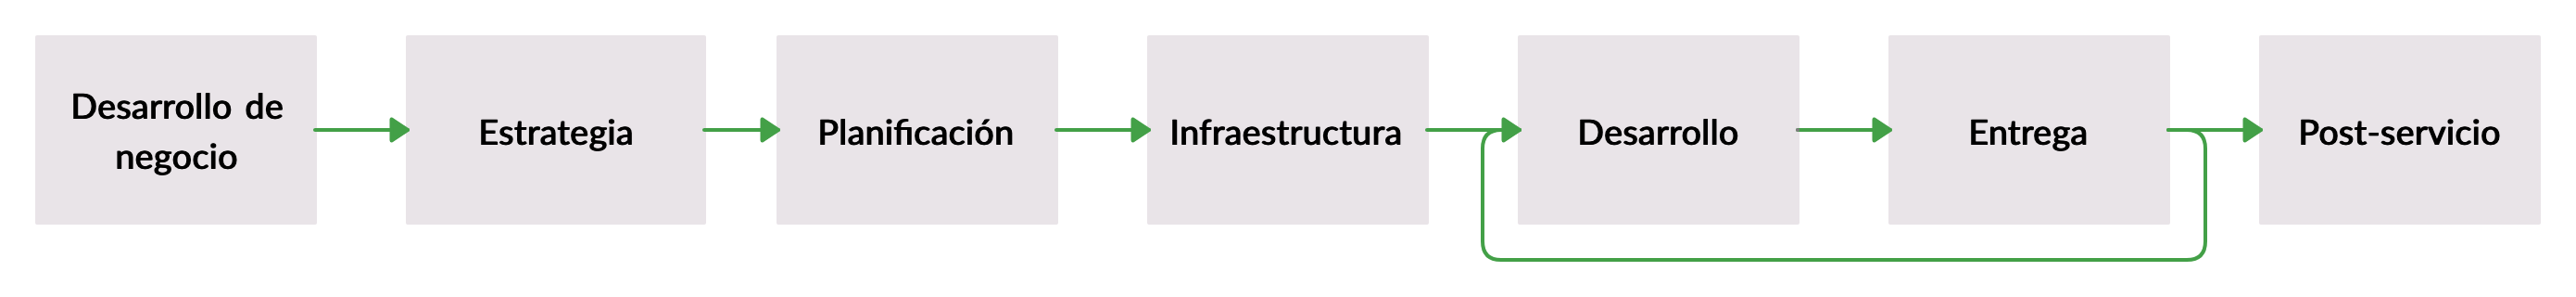
\includegraphics[scale=0.15]{procesos}
    \caption{Diagrama de macroprocesos para proyecto de desarrollo de software}
    \label{fig:procesos}
\end{figure}

La estructura general es adaptable a todo tipo de proyecto que Nursoft ofrezca, a modo de ejemplo, la Figura \ref{fig:consultoria}
ejemplifica la metodología de trabajo para un proyecto de consultoría.

\begin{figure}[h]
    \centering
    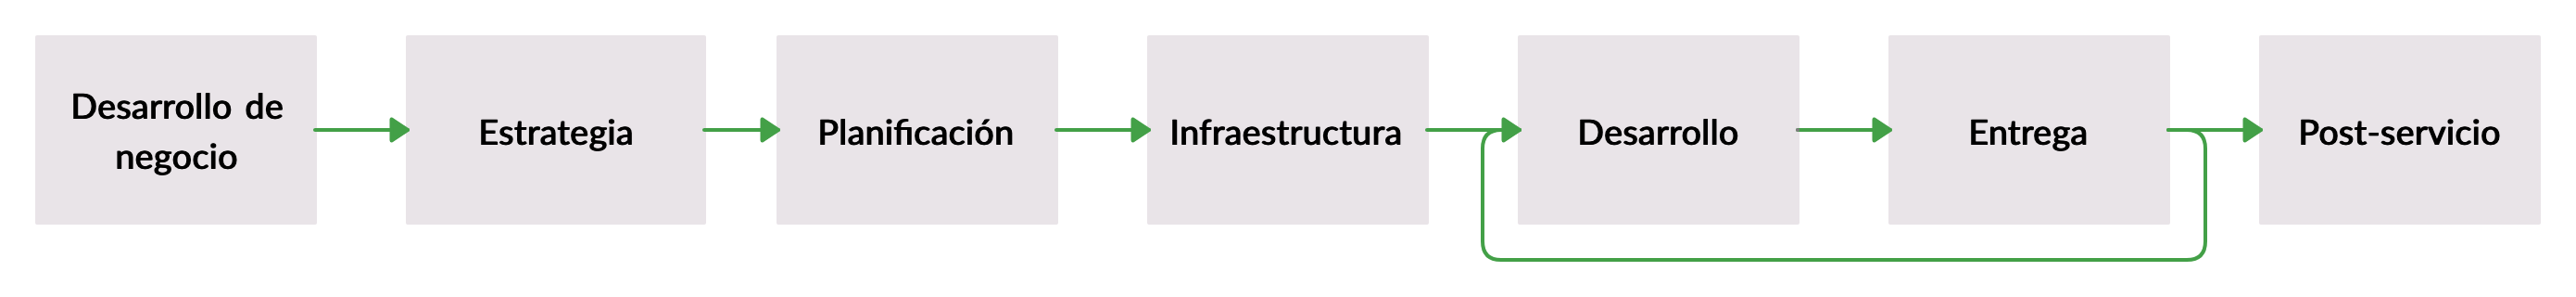
\includegraphics[scale=0.15]{procesos}
    \caption{Diagrama de macroprocesos para proyecto de consultoría}
    \label{fig:consultoria}
\end{figure}


A continuación, se contextualiza brevemente cada macroproceso.

\subsection{Desarrollo de negocio}

El desarrollo de negocio en Nursoft, es el proceso que en una empresa más tradicional se llamaría Venta.
La diferencia es sútil, puesto que Nursoft deja en claro que no vende software como un ítem, vende el desarrollo
de software como una experiencia exclusiva y un servicio altamente flexible y con atención extra al detalle. 
El desarrollo de un negocio implica necesariamente crear una instancia donde ambas partes busquen la mejor parte de
trabajar en conjunto.

En esta etapa se nivelan las expectativas de ambas partes. También se mide la
compatibilidad del cliente con la empresa, con un potencial escenario donde el proyecto no sea aceptado por Nursoft.

Los puntos de mayor importancia de este macroproceso son el levantamiento de necesidades (una versión preliminar de requerimientos),
la creación de la propuesta económica y tecnológica y la firma de contrato. Para el caso de consultorías,
el levantamiento de necesidades se posterga para un macroproceso posterior.

\subsection{Estrategia}

Si la fase de \textbf{Desarrollo de negocios} fue éxitosa, este proceso sigue en el ciclo de vida de un proyecto.

En Nursoft se entiende estrategia como la define Chandler\cite{chandler_1962}:

\begin{displayquote}
Estrategia es la determinación de las metas y objetivos de largo plazo de la empresa,
y la adopción de caminos de acción y de asignación de recursos para alcanzar dichas metas…
\end{displayquote}

En este macroproceso se trabajan cuatro pilares en pos de una visión macro del proyecto:

\begin{itemize}
    \item El cliente
    \item El negocio del cliente
    \item Los usuarios
    \item El software
\end{itemize}

En otras palabras, se define formalmente cuál es el problema o la necesidad del cliente, contextualizada
a elementos internos y externos.

En términos prácticos, en esta etapa participa tanto el departamento comercial como el departamento de diseño
y experiencia de usuario (UX). El primer departamento trabaja para definir directrices de planificación
estratégica a la empresa del cliente (si así lo lo requiera), realizar estudios financieros
para analizar los impactos en el negocio que tendrá el proyecto. 
Al mismo tiempo, el departamento de UX investiga bajo que tipo de interacciones las hipótesis
comerciales del cliente son válidas. Para esto se utilizan diversas metodologías de
investigación del usuario: focus groups, entrevistas y encuestas. 

Este proceso termina con un entregable: la creación de la protopersona\footnotemark[7],
resultado que tendrá un rol protagónico en el siguiente macroproceso.

\footnotetext[7]{La proto-persona es el resultado de contrastar las visiones y expectativas
de un usuario ideal por parte de los \textit{stakeholders} con las expectativas de potenciales
usuarios reales que coincidan con ciertos criterios definidos de los \textit{stakeholders},
por ejemplo rango etario o nivel socioeconómico.}

\subsection{Planificación}

La \textbf{planificación} es el proceso en el cuál se responde qué solución se dará al problema definido en la \textbf{estrategia}.

Esta solución se propone, se investiga y se argumenta tanto desde lo técnico hasta de lo visual.

Por defecto, la planificación cuenta con cuatro fases:
\begin{itemize}
    \item \textbf{Propuesta de solución inicial}
    En la primera propuesta se realizan las mitigaciones técnicas necesarias, y según se necesite se 
    desarrollan los Diagramas de procesos
    \item \textbf{Desarrollo de marca}
    \item \textbf{Diseño y experiencia de usuario}
    \item \textbf{Propuesta de solucion técnica}
    En este último paso, los requerimientos son transformados en Historias de usuarios. Las historias se estiman utilizando la metodología de Planning Poker.
    Utilizando como insumos los entregables de la propuesta inicial, se construye y presenta la propuesta de Arquitectura.
\end{itemize}
\subsection{Infraestructura}
\subsection{Desarrollo}
\subsection{Entrega}
\subsection{Post-servicio}


TODO Insert figura metodologia externa Nursoft.

\begin{itemize}
  \item creación y estandarización de macro-procesos
  \item Ampliar la cartera de grandes clientes 
\end{itemize}


¿Por qué son relevantes estos puntos? El primero se adhiere lógicamente a lo que esta memoria planea
establecer: facilitar y alentar la práctica de registrar esfuerzos, mediante una plataforma especializada,
de la manera más eficiente pero también más lo fiel a la realidad. 
Este proceso es parte de los macro-procesos de Gestión y de Desarrollo. 

TODO: Incluir diagramas de Gestión y Desarrollo

La relevancia del segundo punto no es inmediatamente aparente, por lo que se necesita un poco de contexto.

Desde 2013 hasta antes de la implementación de esta memoria, Nursoft llevaba la gestión básica de sus
proyectos utilizando la plataforma Taiga.
Sus funcionalidades acotadas y simples hicieron un calce perfecto con el Nursoft de ese entonces,
con proyectos de menor escala, y sin muchos procesos formalizados en la parte de gestión. 
Taiga utiliza un lenguaje y una interfaz muy cómoda para desarrolladores y jefes de proyecto,
pero no para \textit{stakeholders} no-técnicos, como clientes y sus asesores.

Adicionalmente, Taiga es una herramienta muy de nicho. De hecho, según Datanyze, su porcentaje de 
porción de mercado es bajísimo, como se muestra en la siguiente tabla:

TODO agregar tabla de Datanyze

¿Qué tiene de relevancia este dato? Nursoft ha descubierto en base a clientes de grandes empresas
con los que trabajó anteriormente, el uso extendido de la plataforma Jira, coincidentemente la plataforma
que mayor cuota de mercado posee.

A mediados de año, Nursoft toma la decisión de cambiar de herramienta de gestión de proyecto a Jira,
pensando en los beneficios de conexión directa con las plataformas de los clientes (si es que las tienen)
https://www.datanyze.com/market-share/project-management/Alexa%20top%201K?page=10

\subsection{Reporte}
Donde se define la estructura de un esfuerzo, en términos de modelado de dato y se contextualiza las partes que componen a un esfuerzo.

\subsection{Herramientas de gestión de proyecto utilizadas}

\textit{Donde se explican brevemente las herramientas externas que se utilizan para llevar
la gestión del proyecto, en términos de historia de usuario, sprints, versiones, etc, y cómo se conectan con la plataforma de reportes}


\paragraph{Taiga} es un gestor de proyectos \textit{open-source}, con un set de funcionalidades
enfocadas en la simpleza y creado para startups, desarrollos ágiles y diseñadores.
Taiga fue liberado en Octubre de 2014 y la última versión fue publicada en Febrero del 2018.

Utiliza \verb|Django| y \verb|Angularjs| para su backend y su frontend, respectivamente.
Cuenta con pocas integraciones \textit{out-of-the-box}, pero soporta
\textit{webhooks}\footnotemark[7] nativamente y cuenta con una API para desarrollar 
integraciones\cite{taiga_webhooks}\cite{taiga_api}.

TODO: Mostrar un proyecto en la plataforma Taiga

\footnotetext[7]{es una estrategia para que dos aplicaciones diferentes se comuniquen, reactivamente, en tiempo real.}

\paragraph{Jira Cloud} es una herramienta propietaria y pagada de gestión de proyectos. 
Puede ser utilizada online o ser descargada e instalada localmente, y fue creada
por la corporación australiana Atlassian. Permite la gestión de proyectos en múltiples metodologías
ágiles como SCRUM, Kanban, e incluso la gestión de proyectos de otras categorías, como post-venta y
solución de errores. 

Es altamente customizable y cuenta con más de 3000 integraciones
externas \cite{jira_features}. Adicionalmente, cuenta con una API para desarrollar integraciones
personalizadas \cite{jira_api}.

TODO: Mostrar un proyecto en la plataforma Jira